% !TeX program = xelatex
% 在 VS Code 中修改 sections/ 内各章；主文件只管理格式和章节顺序。
% 编译：XeLaTeX 两遍；无需 BibTeX、Python 或 ORCA。
\documentclass[UTF8,fontset=fandol,a4paper,11pt]{ctexart}
\usepackage[margin=2.35cm,headheight=14pt]{geometry}
\usepackage{amsmath,amssymb,bm,booktabs,longtable,tabularx,array}
\usepackage{graphicx,float,caption,enumitem,xcolor,fancyhdr}
\usepackage[numbers,sort&compress]{natbib}
\usepackage{hyperref,xurl,microtype}
\definecolor{navy}{HTML}{17324D}
\definecolor{teal}{HTML}{287D8E}
\hypersetup{colorlinks=true,linkcolor=navy,citecolor=teal,urlcolor=teal,
 pdftitle={从工作流到代码生成：面向 ORCA 的闭环自主量子化学计算},
 pdfauthor={BG6022 研究报告}}
\urlstyle{same}
\graphicspath{{figures/}}
\renewcommand{\arraystretch}{1.18}
\setlength{\tabcolsep}{5pt}
\setlength{\emergencystretch}{3em}
\linespread{1.18}
\renewcommand{\topfraction}{0.9}
\renewcommand{\bottomfraction}{0.85}
\renewcommand{\textfraction}{0.08}
\renewcommand{\floatpagefraction}{0.8}
\setlist{nosep,leftmargin=2em}
\captionsetup{font=small,labelfont=bf,labelsep=quad}
\ctexset{section={format=\Large\bfseries},subsection={format=\large\bfseries}}
\pagestyle{fancy}
\fancyhf{}
\fancyhead[L]{\small 面向 ORCA 的自主量子化学计算}
\fancyhead[R]{\small 方法演进与 V4 评估}
\fancyfoot[C]{\thepage}
\newcolumntype{Y}{>{\raggedright\arraybackslash}X}
\newcommand{\Eh}{E_{\mathrm h}}
\newcommand{\code}[1]{\texttt{#1}}
\title{\vspace{-1.2cm}\bfseries 从工作流到代码生成：\\面向 ORCA 的闭环自主量子化学计算\\
 \large BG6022 V2--V4 的方法演进与 V4 系统评估}
\author{}
\date{}
\begin{document}
\maketitle
\vspace{-1.7cm}
% !TeX root = ../main.tex
% 修改摘要内容。
\begin{abstract}
自主量子化学计算需要将科学需求、计算执行与结论验证连接为一致的决策过程。本文以 BG6022 的三个版本为研究对象，依次讨论可追溯固定工作流（V2）、自然语言驱动的工具组合（V3）和证据约束的代码生成（V4）三种思路，并重点研究 V4 的方法设计与实验表现。V2 通过水和乙醇的优化、频率与单点计算建立可复核的计算链；V3 将评价扩展至有限科学任务和对话情境，其固定科学矩阵通过 11/11 个单元，核心基准通过 18/18 个预定义情境。上述成果分别受人工批准、任务定义与对话脚本约束。V4 进一步将任务特定算法交由生成的 Python 和 ORCA 输入表达，以单决策循环、目标与计划分离、统一执行入口及累计预算约束开放任务。早期乙醇案例实现自主优化与频率分析，含人工元数据协助的正己烷案例获得四个候选的单点能量排序。按 ORCA 正常结束判定计算成功，V4 已在乙醇优化与频率、正己烷候选能量、正丁烷部分扫描点、丙酮激发态、气相与水环境能量比较以及 HCN 屏蔽张量六类任务中取得数值结果；甲醛极化率尚无结果。原七任务冻结批次的 8 次 ORCA 启动中，7 次计算成功（87.5\%）；后续成功案例按各自批次和实际理论水平分别报告。乙醇优化获得 21 个正频率且无虚频，两种基组下水环境相对气相的电子能差分别为 $-18.276507$ 和 $-16.607972$ kJ mol$^{-1}$。研究表明，生成代码能够支持多种量子化学任务的真实执行，几何对应、结果提取与完整交付仍需进一步完善。三个版本反映研究问题的递进，现有数据不构成共同基准上的性能排序。
\end{abstract}

\noindent\textbf{关键词：}自主量子化学；大语言模型；ORCA；工具组合；代码生成；闭环决策；科学验证


% !TeX root = ../main.tex
\section{引言}
电子结构计算为分子结构、光谱与反应性研究提供了重要工具。密度泛函理论（density functional theory, DFT）通过电子密度描述基态多电子体系，Kohn--Sham 方案使其能够转化为实际可求解的自洽问题\cite{hk,ks}。然而，计算软件能够完成某种求解，并不意味着研究者的科学问题已经得到回答。方法和基组选择、电荷与自旋设定、结构准备、收敛诊断以及结果解释共同决定计算的有效性。

传统自动化主要将已知计算协议转化为可重复执行的流程。大语言模型则提供了进一步连接自然语言需求、软件知识与程序生成的可能性。ReAct、Toolformer 与 Reflexion 分别从推理与行动交替、工具使用及反馈修正等角度发展了语言模型 Agent 的方法基础\cite{react,toolformer,reflexion}。ChemCrow 和 Coscientist 展示了模型调用化学工具、组织化学研究操作的可行性\cite{chemcrow,coscientist}。对于量子化学，这一方向的关键问题已从“能否生成输入”扩展为“能否保持科学目标，并根据中间证据组织后续计算”。

本文沿 BG6022 V2、V3、V4 的顺序考察三种研究思路。V2 聚焦计算链的可追溯性，首先建立受控执行与证据复核的基础。V3 将研究对象扩展到有限任务范围内的自然语言交互和工具组合。V4 则将任务特定算法的生成置于中心，研究如何在统一工具边界内，以生成代码处理更开放的科学目标。该顺序表示研究重心的变化，不预设后续版本在所有任务上具有更高成功率。

V4 是本文的主要研究对象。系统采用 ORCA 及 ORCA Python Interface（OPI）作为科学计算基础\cite{orca2020,orca6,opipaper}，使用单一决策循环组合通用工具与现场代码，并将原始目标、实际执行、科学检查和结果交付分别记录。本文的贡献包括：建立三个版本之间的研究问题联系；阐述 V4 的目标保持与受控代码执行机制；通过科学案例和跨任务评测分析执行成功与完整目标完成之间的差异。本文关注自主计算系统的方法与验证，不提出新的电子结构近似。


% !TeX root = ../main.tex
\section{相关工作与评价基础}
\subsection{计算工作流与闭环科学 Agent}
ASE、AiiDA、Atomate2 和 cclib 分别发展了原子模拟接口、来源可追溯工作流、模块化计算流程及统一输出解析\cite{ase,aiida,atomate2,cclib}。这些方法说明，标准化执行与数据组织本身就是科学自动化的重要组成部分。语言模型的引入增加了需求解释、候选操作选择和任务代码生成能力，但并不替代既有数值算法、程序适配或科学检查。

AutoDFT 将战略规划、即时参数规划、监控、恢复、反思与后处理组织为多角色闭环。在包含 34 个任务和 9 类计算的 VASPBench 上，原文表 1 报告完整系统、开环系统和规则基线分别完成 32、28 和 23 个任务；性质评价另采用 20 个材料，并在成功计算上统计误差\cite{autodft}。其主要启发是：成功结果同样需要进入反馈过程，因为新的结构或物性信息可能改变后续计算需求。相关数字对应论文自身的软件、任务和单次运行设置，不作为本文系统的直接性能参照。

Lee 与 Rondinelli 研究基于 ORCA 的自主多参考计算，采用 CASSCF/SC-NEVPT2 与 aug-cc-pVTZ。在 558 个跃迁目标中，基线、决策阶梯和完整信息复制设置分别覆盖 139、246、378 个目标，对应已确认电子态子集的 MAE 为 0.373、0.339、0.023 eV\cite{multirefagent}。不同设置的误差分母并不相同，完整信息复制还使用更充分的先验协议。该研究进一步表明，数值收敛、电子态身份与目标覆盖必须分别评价。

CASSCF 需要明确活性空间，NEVPT2 在多参考波函数基础上补充动态电子相关\cite{casscf,nevpt2}；AVAS 等方法为自动构建活性轨道提供了专门算法基础\cite{avas}。QUESTDB 则提供激发能参照\cite{questdb}。这些研究对本文的意义在于界定科学验证问题，而非证明 BG6022 已具备多参考自主求解能力。本文不将尚未经实际验证的活性空间选择或态识别列为 V4 成果。

\subsection{方法条件与科学含义}
固定核构型下，Kohn--Sham 电子能泛函可写为
\begin{equation}
E[n]=T_{\mathrm s}[n]+\int v_{\mathrm{ext}}(\bm r)n(\bm r)\,\mathrm d\bm r
+E_{\mathrm H}[n]+E_{\mathrm{xc}}[n].
\end{equation}
分子势能还需加上核间排斥能。交换相关近似、基组、色散处理和几何均影响实际求解；PBE、Becke 杂化方案、LYP 相关泛函、def2 基组及 D3 色散修正代表相关方法选择\cite{pbe,becke,lyp,def2,d3}。本文各案例按实际使用的理论水平报告，不以不同方法的绝对能量差评价准确度。

含时密度泛函理论为激发态计算提供理论基础\cite{tddft}，CPCM 等连续介质方法则用于描述环境效应\cite{cpcm}。因此，“计算能量”不足以唯一确定科学任务：基态或激发态、气相或溶液、固定几何或优化几何均需明确。构象问题还涉及采样范围；GFN2-xTB 和 CREST 为低成本势能描述与构象集合搜索提供了专业方法\cite{gfn2,crest}。本文正己烷案例实际使用力场候选与 DFT 单点，上述文献仅说明相关研究背景。

\subsection{计算成功的定义与科学解释}
本文以 ORCA 原始输出的正常结束记录作为计算成功判据，记 $X_i=\text{正常结束}$ 为成功；未启动的调用记为未计算，异常结束记为计算失败。对已启动调用，计算成功比例为 $N_{\mathrm{normal}}/N_{\mathrm{started}}$。科学结论按所获证据另行解释。令 $X_i$ 表示第 $i$ 次计算的执行事实，$S_{ik}$ 表示其第 $k$ 个输出的科学检查，$G_j$ 表示第 $j$ 个必需目标是否满足。三种状态分别为
\begin{equation}
X_i=\text{正常结束},\qquad
S_{ik}=\text{通过规定检查},\qquad
G_j=\text{目标证据充分}.
\label{eq:states}
\end{equation}
正常结束可能产生未经验证的观察；已验证单点能量也不能替代优化自由能或完整势能扫描。完整任务还要求必需交付项齐备：
\begin{equation}
C_{\mathrm{task}}
=\left(\bigwedge_{j\in\mathcal G_{\mathrm{required}}}G_j\right)
\land D_{\mathrm{required}}.
\label{eq:complete}
\end{equation}
这一表达强调评价语义，并不意味着所有科学问题具有相同检查清单。

存在独立参考时，覆盖率和误差应共同报告：
\begin{equation}
\mathrm{Coverage}=\frac{N_{\mathrm{matched}}}{N_{\mathrm{target}}},
\qquad
\mathrm{MAE}_{\mathrm{matched}}
=\frac{1}{N_{\mathrm{matched}}}\sum_{i\in\mathcal M}
|E_i-E_i^{\mathrm{ref}}|.
\end{equation}
$\mathcal M$ 仅包含可确认对应关系的目标。本文的系统评测主要检验执行、收敛、来源与目标交付；没有独立高精度参考的任务不报告数值 MAE。可追溯数据有助于复核和复用\cite{fair}，但文件完整性不等于物理结论正确。

% Chronological predecessor studies; statistics are version-scoped.


% !TeX root = ../main.tex
\section{V2：以过程一致性为中心的可追溯工作流}
\label{sec:v2}
\subsection{研究思路}
V2 首先处理实际科学计算中过程与证据的一致性问题。其基本组织方式是将已知计算协议分解为明确步骤，在受控启动、状态保存和产物关联的基础上形成可复核计算链。模型决策并非这一阶段量化成果的主要来源；研究重点在于确认计算确实发生、原始结果得到保留，并能够在不重算的情况下恢复其科学含义。

这一设计对应自主计算的基础要求：若输入几何、实际执行条件或输出来源不能被可靠识别，即使后续加入语言模型，也难以判断模型所使用的数值是否属于正确任务。因此，V2 将真实执行与离线科学重解析分离，以固定结果验证证据保存和解释的一致性。

\subsection{计算结果}
本文采用两条人工逐节点批准的成功计算链作为 V2 案例。水和乙醇均使用 ORCA 6.1.1、气相、零电荷、单重态及 r$^{2}$SCAN-3c/TightSCF，执行优化、频率和单点计算。r$^{2}$SCAN-3c 是具有组合校正的复合电子结构方法\cite{r2scan3c}。后续科学分析读取已有输出，没有启动重复计算。结果见表 \ref{tab:v2} 和图 \ref{fig:v2-convergence}。

\begin{table}[htbp]
\centering\small
\caption{V2 两条受控计算链的结果。耗时为 ORCA 各节点自报经过时间之和，未包含人工等待及工作流开销；不同分子和核数不用于计算加速比。}
\label{tab:v2}
\begin{tabularx}{\linewidth}{p{5.3cm}YY}
\toprule
指标 & 水 H$_2$O & 乙醇 C$_2$H$_6$O\\
\midrule
核数 / 总内存 / MaxCore & 1 / 2048 MB / 1536 MB & 4 / 2048 MB / 384 MB\\
成功计算节点 & Opt、Freq、SP 各一次 & Opt、Freq、SP 各一次\\
优化周期 & 4 & 11\\
优化末次评价电子能 / $\Eh$ & $-76.418938721015$ & $-155.002314096955$\\
后续单点电子能 / $\Eh$ & $-76.418938721035$ & $-155.002314094574$\\
首周期至优化终态降能 / m$\Eh$ & 1.692636839 & 7.859199377\\
正振动模式数 & 3 & 21\\
正频率范围 / cm$^{-1}$ & 1653.249--3932.735 & 248.134--3837.522\\
三节点自报总耗时 / s & 24.143 & 98.855\\
\bottomrule
\end{tabularx}
\end{table}

\begin{figure}[htbp]
\centering
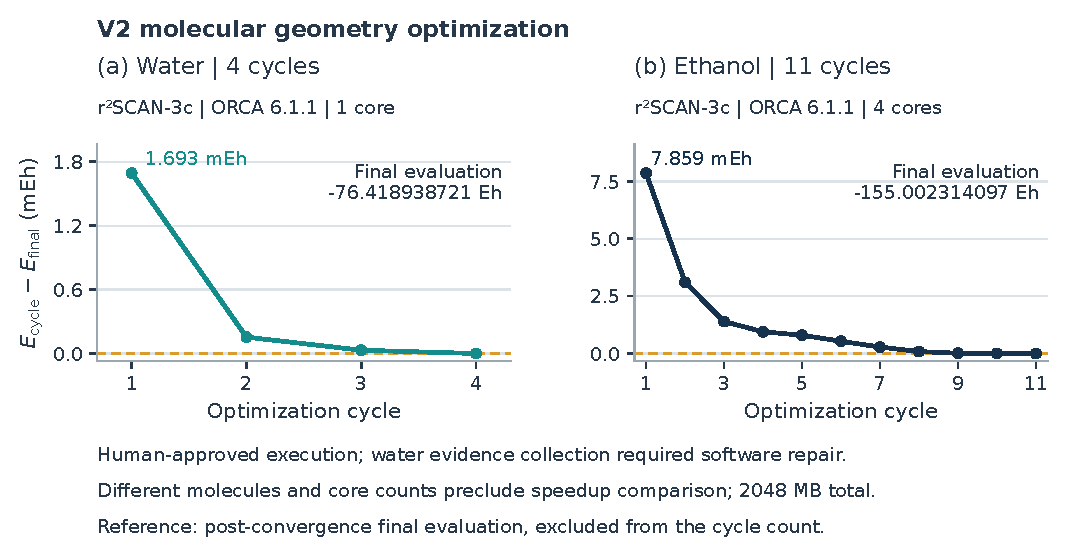
\includegraphics[width=\linewidth]{v2-optimization.pdf}
\caption{V2 水与乙醇的优化收敛曲线。纵轴为各周期电子能减去对应优化末次评价能量，单位 m$\Eh$。收敛后的末次评价仅提供零点，不额外计作优化周期。}
\label{fig:v2-convergence}
\end{figure}

水与乙醇分别获得 3、21 个正振动模式，历史检查支持其给定理论水平下的局部极小值。定义 $\Delta E=E_{\mathrm{SP}}-E_{\mathrm{Opt,final}}$，两者的内部重复评价差分别为 $-2.0\times10^{-11}\,\Eh$ 与 $2.381\times10^{-9}\,\Eh$。该差值反映同一终态的数值一致性，而非相对实验或高精度参考的误差。

\subsection{方法边界与后续问题}
上述成果建立了实际计算与证据复核的可行性，但不构成无人干预的成功率估计：两条链经过人工批准，水链的结果采集还包含开发者修正。单一初始构型也不能支持全局构象结论。V2 因此提供的是可靠操作与可复核证据的基础，而尚未检验自然语言需求如何自主转化为组合计算。后者构成 V3 的主要研究问题。


% !TeX root = ../main.tex
\section{V3：有限任务范围内的语义驱动工具组合}
\label{sec:v3}
\subsection{研究思路}
V3 将研究对象从固定计算链扩展到自然语言交互与工具组合。系统在已定义的科学能力范围内解释需求，建立结构化请求，并通过组合工具完成单点、优化、频率和派生量分析。相较 V2，其重点从过程保存转向用户语义与可执行操作之间的连接。

这一思路将科学求解能力主要保留在既有工具中，模型参与语义规范化、结果回答和有限修复。因而，V3 的评价既需验证基础工具的科学输出，也需考察对话情境中的条件修改、已有结果查询、澄清、拒绝与失败恢复。两类评价应区分统计。

\subsection{固定科学矩阵}
Scientific Matrix v1 在 5 类任务与 6 个分子对象中显式选择 11 个单元，11/11 单元通过，实际 ORCA 为 16 次、模型调用为 0，整体经过时间为 421.516 s。该矩阵采用固定请求和计划，检验组合执行与科学检查，不作为模型驱动端到端能力的证据。覆盖范围和部分科学结果见图 \ref{fig:v3-matrix}、表 \ref{tab:v3-science}。

\begin{figure}[htbp]
\centering
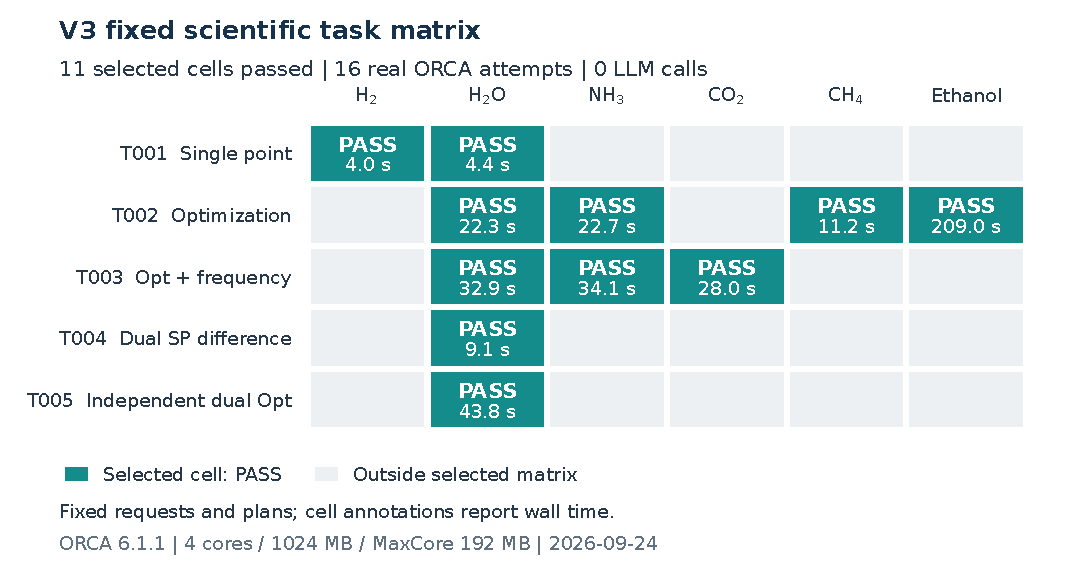
\includegraphics[width=\linewidth]{v3-scientific-matrix.pdf}
\caption{V3 固定科学矩阵。11 个启用单元全部通过，灰格未纳入评价分母。单元内标注经过时间；该批次使用真实 ORCA，模型调用为 0。}
\label{fig:v3-matrix}
\end{figure}

\begin{table}[htbp]
\centering\small
\caption{V3 科学矩阵的优化与频率结果。理论水平为气相 r$^{2}$SCAN-3c、零电荷、单重态，资源为 4 核、1024 MB、MaxCore 192 MB/进程。}
\label{tab:v3-science}
\begin{tabularx}{\linewidth}{p{1.8cm}rp{4.6cm}Y}
\toprule
分子 & 优化周期 & 最终优化电子能 / $\Eh$ & 相应频率检查\\
\midrule
H$_2$O & 5 & $-76.418938720985$ & 3 个正模式，局部极小值支持\\
NH$_3$ & 5 & $-56.541874067217$ & 6 个正模式，局部极小值支持\\
CO$_2$ & 3 & $-188.570062871358$ & 4 个正模式，局部极小值支持\\
CH$_4$ & 2 & $-40.494915367074$ & 仅优化，未作频率结论\\
乙醇 & 36 & $-155.002354316872$ & 仅优化，未作频率结论\\
\bottomrule
\end{tabularx}
\end{table}

水的三个正振动频率为 1653.24、3813.59、3932.75 cm$^{-1}$；CO$_2$ 为 668.14、668.14、1362.20、2422.54 cm$^{-1}$。线性 CO$_2$ 的五个外部零模式与四个振动模式被分别检查。两次固定矩阵记录的对照中，13 个电子能结果在输出的 12 位小数精度上相同，三套频率一致。这支持指定输入和设置下的数值重复性，不替代外部准确度评价。

\subsection{模型参与的核心基准}
Benchmark 1.2 core 的最终评分为 18/18，其分母包括 11 个固定科学题、5 个脚本化对话情境和 2 个名称解析题。16 项实际涉及计算，另两项为澄清与拒绝。实验驱动发送预定义话语，并在公开确认状态发送确认回复，经系统的正常对话入口执行，没有直接注入规范请求或计划。

该批次使用 DeepSeek Flash，共 37 次模型调用：语义规范化 19 次、结果回答 17 次、修复 1 次；专门 Intake/Planner 模型调用均为 0。输入、输出和总 tokens 分别为 140,953、6,985 和 147,938，整体经过时间为 667.547 s。ORCA 共尝试 23 次，包括 22 次成功和 1 次预设受控失败，随后执行一次有界修复。图 \ref{fig:v3-cost} 给出调用与耗时分布。

\begin{figure}[htbp]
\centering
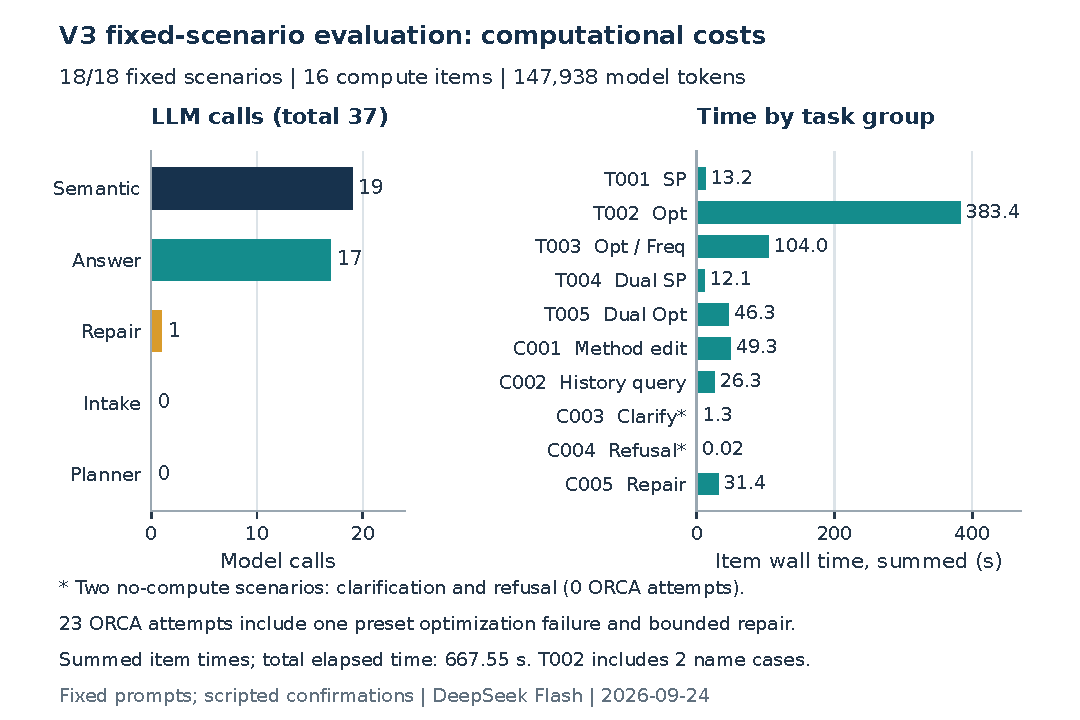
\includegraphics[width=\linewidth]{v3-core-costs.pdf}
\caption{V3 核心基准的模型调用分工与任务组耗时。18/18 表示预定义情境的最终评分，其中两项不执行计算；23 次 ORCA 尝试包含一次预设失败及其后续修复。各组的对象和步骤数不同，耗时不作效率排序。}
\label{fig:v3-cost}
\end{figure}

受控失败通过限制优化迭代次数产生，用于检验已定义修复路径，不能解释为自然故障发生率。最终评分还对一项确定性拒绝情境作过规则校准，保存观察没有重跑。因此，18/18 应理解为有限范围内的情境评分，而非任意自然语言任务的自主成功概率。

\subsection{方法边界与 V4 的研究动机}
V3 说明，自然语言语义、工具执行和有界修复可以在有限任务集合中协同运行。然而，科学题的方法、结构和目标受到预定义条件约束，对话也由脚本组织；完整扩展集与未见任务集未运行，数值结果未相对外部高精度参照评价。这些限制使现有成果主要支持已定义范围内的组合能力。

在此基础上，新的问题是：当科学需求要求已有工具未封装的采样、分析或算法时，是否必须由开发者增加专用求解模块？本文据此将 V4 的研究重点转向任务算法的现场生成，通过固定通用工具与生成代码的组合拓展任务表达，同时保持执行边界和科学验证要求。该过渡是基于已有证据的研究问题重构，不构成版本性能提升的预先结论。


% !TeX root = ../main.tex
\section{V4：证据约束的代码生成与单循环决策}
\label{sec:v4-method}
\subsection{研究问题与总体结构}
V3 的有限任务结果尚未回答一个更开放的问题：当用户需求不能由既有工具中的固定算法直接表达时，系统能否生成新的任务程序，并保持原始科学目标与验证条件？V4 以此为中心，将任务表达从工具参数扩展到现场生成的 Python 和 ORCA 输入。Code as Tools 的基本原则是：任务特定算法由代码表达，通用工具承担校验、执行和产物管理。

V4 采用一个决策主循环。模型根据当前目标、计划和证据提出下一动作；程序检查依赖、资源和执行边界后调用工具；新结果先接受科学检查与目标评价，再反馈至下一轮决策。计算正常结束后仍可能需要精度检查、补充采样或跨结果分析，失败则可能引出输入修复或有原因的停止。该组织不预设优化、频率与单点的固定顺序。

\begin{figure}[H]
\centering
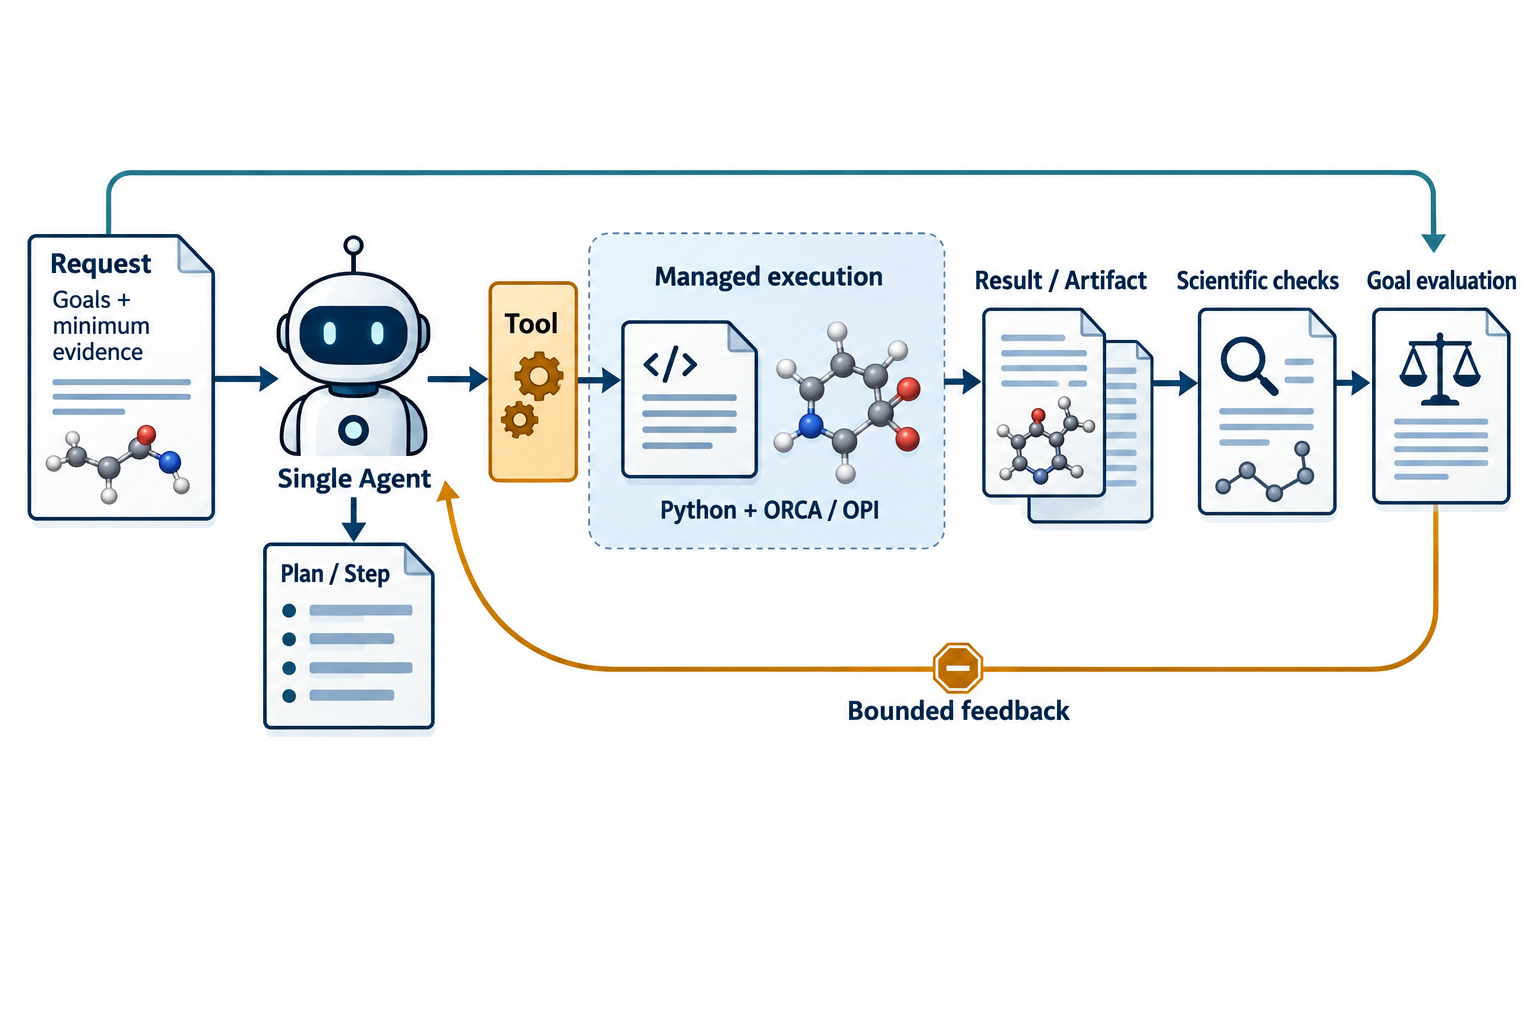
\includegraphics[width=\linewidth,trim=14 205 14 112,clip]{method-overview.png}
\caption{V4 的证据约束闭环。原始目标独立约束结果评价；单一决策者通过工具边界组织计算，依据新证据修订执行路线。该图为方法示意。}
\label{fig:architecture}
\end{figure}

\subsection{领域表示与目标保持}
系统采用 Request、Plan、Step、Tool、Run、Result 和 Artifact 七类长期对象，分别表达科学需求、实现路线、具体步骤、执行接口、运行过程、结果与证据产物。表 \ref{tab:objects} 给出其功能关系。该表示将目标语义、执行状态和科学结果分离，避免由单一“成功”标记覆盖不同层次的事实。

\begin{table}[htbp]
\centering\small
\caption{V4 的核心表示及其方法作用。}
\label{tab:objects}
\begin{tabularx}{\linewidth}{p{1.8cm}YY}
\toprule
对象 & 主要内容 & 方法作用\\
\midrule
Request & 科学对象、物理量、条件、最低证据 & 固定任务所要回答的问题\\
Plan & 步骤依赖、目标到证据的路线 & 允许调整实现策略\\
Step & 工具参数、输入或代码版本 & 明确一次具体操作\\
Tool & 接口约束、执行影响、检查与产物 & 建立可验证的执行边界\\
Run & 配置、尝试、资源与累计用量 & 保持运行连续性与有限成本\\
Result & 执行事实、科学检查、观察与目标评价 & 区分结果层次\\
Artifact & 几何、输入、程序、原始输出与来源 & 支持追溯和复核\\
\bottomrule
\end{tabularx}
\end{table}

目标和最低证据保存在 Request 中，Plan 仅负责实现路线。例如，将“在同一几何上比较气相与水环境能量”修订成两套独立优化，虽然可能产生两个数值，却改变了原问题。不同目标允许具有不同环境或电子态，实际执行条件因而需要按目标匹配，而不能无条件归并为全局设置。

修复同样受到目标保持约束。当某个程序因语法或输入错误而修改时，未改变的目标路线应保持关联；修复不能通过删除目标或降低最低证据要求获得形式上的完成。用户明确条件、默认值、继承条件与自动选择分别记录，以便区分模型决策和外部约束。

\subsection{统一执行入口与任务算法生成}
V4 支持三种输入形式：OPI 构造的输入、原生 ORCA 输入，以及生成 Python 通过薄接口发起的内部计算请求。三者复用相同的 ORCA 执行管理与既有解析、检查链，OPI 接口行为以其版本化文档为依据\cite{opi}。薄接口负责请求计算和返回产物引用，不内置构象搜索、势能扫描等具体解题算法。

因此，开放性主要来自任务程序的组合能力。一个程序可以构建几何集合、选择有限候选、提交内部计算，并在结果产生后执行确定性分析。相同通用工具可被用于不同性质或数据组织方式，减少为每个问题增加专用求解接口的需要。这一机制扩展的是表达能力，其科学有效性仍需按输出检查。

模型负责提出意图、参数、代码和修复建议，程序负责判定是否可执行。生成代码不能自行扩展权限、修改系统实现或宣告科学通过。工具目录、参数定义、执行校验与输出声明保持一致，以减少规划接口与实际行为之间的不一致。

\subsection{开放观察与科学资格}
新任务可能产生尚未纳入标准检查的性质。V4 允许代码从原始输出提取此类数据，并将其记录为带来源、单位和验证说明的观察。这有助于支持开放分析，但观察不会自动成为经过科学检查的正式结果。程序退出码、字段存在或脚本给出的“通过”均不足以替代性质相关验证。

对于标准检查已覆盖的输出，系统沿用统一解析与科学检查；对于未覆盖的输出，则披露其证据状态及结论边界。是否足以满足目标取决于原请求的最低要求，而不是模型对结果的主观评价。该区分尤其适用于激发态、张量性质和由多个计算派生的结论。

原始输入、初始几何和历次尝试保持独立；结果引用通过内容校验绑定相应产物。读取已有证据不隐式触发转换或重算，额外分析和补算作为明确操作进入决策过程。这样既保留失败事实，也使成功结果能够被后续步骤可靠消费。

\subsection{有界反馈、资源与停止机制}
开放代码引入了动态计算数量与程序行为，因此资源与预算需要覆盖整个任务，而不只约束最外层调用。对预算维度 $k$，令上限为 $B_k$、累计用量为 $U_k$、新动作预留为 $r_k$，执行前要求
\begin{equation}
U_k+r_k\leq B_k.
\end{equation}
内部 ORCA 调用、代码重试与模型纠错均计入累计用量；运行恢复不重置消耗。执行状态不明时先核对既有运行事实，避免重复启动。

生成程序及其科学子进程处于受管理的执行范围中，共同受到计算资源、文件访问和通信约束。本文评估所采用的环境计算并发为 1，使用 4 核、进程树内存上限 1024 MiB 和 ORCA MaxCore 192 MiB/进程。MaxCore 是程序内部参数，不能替代总内存限制。既有隔离测试仅支持已评估配置，不能推导任意环境下的安全性。

反馈内容需在有限上下文内同时保留原始目标、当前结果和有效修复信息。V4 采用当前证据摘要与可查询来源相结合的组织方式。预算耗尽、证据不足或不适用均可构成停止理由；停止后已经正常结束的 ORCA 调用保留计算成功标记，其科学解释与工作流交付状态分别记录。


% !TeX root = ../main.tex
\section{V4 的实验设计与结果}
\label{sec:v4-eval}
\subsection{实验范围与评价层次}
V4 的证据分为执行环境验证、模型驱动科学案例、辅助完成案例和冻结跨任务评测。执行环境验证检验受管理入口能否启动与收集实际计算；科学案例考察特定自主路线；跨任务评测检验从需求到必需交付的完整性。各项结果以产生证据时的实现配置为准。本文以 ORCA 正常结束为计算成功的主要指标，并列出实际能量、频率及响应性质；完整工作流交付作为附加指标，后续补充案例不混入冻结批次的分母。

跨任务评测采用七项请求：乙醇优化与频率、正己烷构象、正丁烷扭转扫描、丙酮五个激发态、气相与水环境能量比较、HCN 核磁屏蔽、甲醛极化率旋转比较。每项在所评估配置下运行一次，计算、提示和评价设置在运行期间保持固定。后两项在后续实验中已暴露，应视为回归任务。

\begin{table}[htbp]
\centering\small
\caption{本文纳入的 V4 主评测条件。该设置与早期科学案例的模型和参数分别记录。}
\label{tab:v4-settings}
\begin{tabularx}{\linewidth}{p{4.4cm}Y}
\toprule
项目 & 评测设置\\
\midrule
科学计算程序 & ORCA 6.1.1；OPI 2.0.0\\
模型标识 & DeepSeek Flash，低推理强度设置\\
任务数 / 每任务尝试 & 7 / 1\\
计算资源 & 4 核；1024 MiB；MaxCore 192 MiB/进程；并发 1\\
期限 & 单次 ORCA 900 s；父 Python 1200 s；总任务 7200 s\\
输入上下文上限 & 64000 的配置容量上限\\
主要评价 & ORCA 正常结束及实际数值结果；附加记录科学检查与交付\\
独立数值参考 / 完整重复 & 该评测未进行\\
\bottomrule
\end{tabularx}
\end{table}

评测保留每次模型响应、计算尝试与原始结果；失败后不另建独立运行选择成功样本。早期案例中的人工协助另行披露。不同实验配置和任务暴露使跨批次数据无法视为同版本独立重复，因此本文主要采用描述性统计与案例分析。

\subsection{执行验证与乙醇自主案例}
执行环境验证覆盖 21 种不同情境，累计包含 8 次实际 ORCA 启动和 0 次模型调用。固定水分子 RHF/STO-3G 单点与严格优化分别得到 $-74.96299161531729\,\Eh$ 和 $-74.96590119219361\,\Eh$。这些数据支持指定执行路径的可用性；未包含频率分析的优化不被解释为极小值证据。

早期乙醇模型驱动案例选择 B3LYP/def2-SVP、气相、零电荷、单重态的 RKS 设置，以一次 Python 和一次四进程 ORCA 计算完成优化与频率分析。模型标识为 DeepSeek V4 Pro，低推理强度，共 17 次请求和 224,492 tokens。独立科学复核结果见表 \ref{tab:v4-ethanol}。

\begin{table}[htbp]
\centering\small
\caption{V4 乙醇自主案例的科学复核。结论限于给定理论水平与所得构型。}
\label{tab:v4-ethanol}
\begin{tabularx}{\linewidth}{p{5.6cm}Y}
\toprule
指标 & 结果\\
\midrule
最终电子能 & $-154.828249797040\,\Eh$\\
原子数 / 全部模式 & 9 / 27\\
模式分类 & 6 个外部零模式，21 个正振动模式\\
最低正频率 / 最高频率 & 276.1200 / 3804.5901 cm$^{-1}$\\
几何独立复核最大差 & $6.91\times10^{-9}$ \AA\\
Hessian 重建频谱最大差 & $2.1624\times10^{-4}$ cm$^{-1}$\\
收敛条件 & 五项优化阈值、SCF 及 27 个 CP-SCF 扰动通过\\
结果状态 & 两个目标满足；ORCA 计算成功；独立复核支持局部极小值\\
\bottomrule
\end{tabularx}
\end{table}

该复核支持所得构型为局部谐振极小值。系统当时仍将相关产物记录为未经正式资格检查的观察，独立复核没有追溯改变原始状态。因此，本例既提供一条自主科学路线的正面证据，也说明外部复核与系统内正式资格覆盖应分别评价。该案例没有提供全局构象结论、运行失败后修复成功或多次重复可靠性的证据。

\subsection{有限正己烷候选比较}
另一案例使用生成代码构造并保存 12 个候选，在四次 ORCA 限额内选择其中 4 个进行 B3LYP/6-31G、RKS、气相、零电荷、单重态单点计算。相对能量定义为
\begin{equation}
\Delta E_i=(E_i-\min_{j\in\mathcal S}E_j)
\times2625.4996394799\ \mathrm{kJ\,mol^{-1}}/\Eh,
\end{equation}
其中 $\mathcal S$ 仅含已评估四个候选。图 \ref{fig:conformers} 给出结果。

\begin{figure}[htbp]
\centering
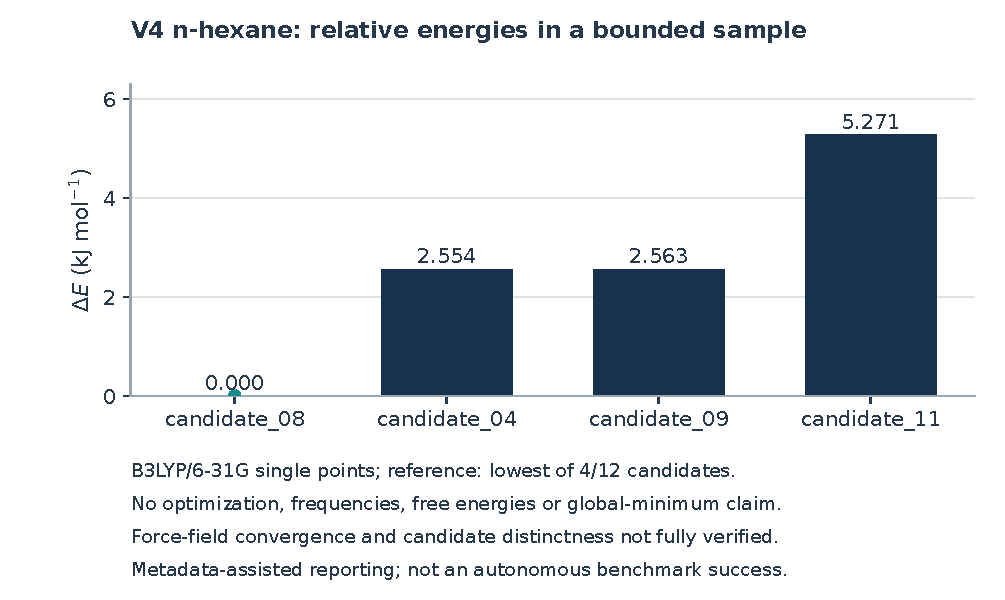
\includegraphics[width=0.94\linewidth]{bounded-conformers.pdf}
\caption{V4 正己烷有限候选的单点相对电子能。四个已评估候选相对于子集最低值为 0、2.554112、2.563181、5.270516 kJ mol$^{-1}$。另八个候选未进行 ORCA 计算，所得顺序不代表全局构象、自由能或极小值排序。}
\label{fig:conformers}
\end{figure}

任务代码与科学计算来自模型驱动过程，最终证据组织与交付包含人工元数据协助及分次续作。相关运行累计 38 次模型请求、854,725 tokens 和 4 次 ORCA 计算，不能计入完全自主冻结评测的成功样本。候选间完全互异与力场收敛也未充分验证。本例支持预算内有限候选比较的可行性，其证据边界不同于全局构象搜索。四次 ORCA 单点均作为计算成功记录。

% !TeX root = ../main.tex
\subsection{已成功计算的任务与数值结果}
\label{sec:successful-results}
为完整呈现实际计算产出，本节进一步汇总后续修复实验及历史批次中的成功计算。本文将原始输出含 ORCA 正常结束记录的调用标注为\textbf{计算成功}，并另行说明收敛、几何及性质解释的证据范围。T1--T5 与 H1 六类任务已有数值结果，H2 尚无极化率结果。这里的六类覆盖来自不同配置与多次开发尝试，不能解释为同一版本七题一次运行的成功率；它也不改变各历史批次的原始工作流完成记录。

\begin{table}[htbp]
\centering\small
\caption{V4 已获数值结果的任务覆盖。成功按实际 ORCA 调用判断，附加说明限定结论范围。}
\label{tab:successful-coverage}
\begin{tabularx}{\linewidth}{p{0.9cm}p{2.2cm}p{2.2cm}Y}
\toprule
任务 & 计算状态 & 主要批次 & 已获得结果\\
\midrule
T1 & 计算成功 & a010 & 乙醇优化能量、收敛结构与 21 个正频率\\
T2 & 计算成功 & a005、a007 & 两批共 10 个候选的单点能量及批内排序\\
T3 & 计算成功（部分点） & 第三冻结批次 & 六个约束优化计算点；角度对应待核查\\
T4 & 计算成功 & 第一冻结批次 & 丙酮五个单重态激发能及振子强度\\
T5 & 计算成功 & a026、a027 & 两种基组下各一对气相与 CPCM 水能量\\
H1 & 计算成功 & a011 & 三核总屏蔽张量及各向同性屏蔽\\
H2 & 尚无计算结果 & 已有记录 & 未获得两个取向的静态极化率\\
\bottomrule
\end{tabularx}
\end{table}

\subsubsection{T1：乙醇优化与振动频率}
批次 a010 使用气相 r$^{2}$SCAN-3c 及其内置 def2-mTZVPP 基组，电荷为 0、多重度为 1。ORCA 计算成功，优化的五项数值收敛阈值均满足，最终电子能为 $-155.002345492244\,\Eh$。27 个模式中包含投影后的 6 个平动和转动零模式、21 个正振动模式及 0 个虚频。全部正频率见表 \ref{tab:t1-frequencies}。这些结果支持该理论水平下的局部极小值，不证明全局最低构象。

\begin{table}[htbp]
\centering\small
\caption{a010 乙醇的 21 个正振动频率，单位 cm$^{-1}$，按 ORCA 打印精度列示。}
\label{tab:t1-frequencies}
\begin{tabular}{rrrrrrr}
\toprule
270.90 & 298.95 & 425.86 & 811.51 & 882.13 & 1052.13 & 1066.45\\
1134.41 & 1282.25 & 1371.13 & 1396.18 & 1418.25 & 1483.33 & 1487.57\\
1509.53 & 2969.59 & 3004.65 & 3061.83 & 3088.36 & 3105.66 & 3819.31\\
\bottomrule
\end{tabular}
\end{table}

\subsubsection{T2：正己烷有限候选的单点能量}
a007 和 a005 分别完成 6 次与 4 次气相 r$^{2}$SCAN-3c 单点计算，均为中性单重态。表 \ref{tab:t2-energies} 给出真实电子能及相对能量；每批以各自已计算子集的最低能量为参考，换算采用 $1\,\Eh=2625.4996394799$ kJ mol$^{-1}$。候选编号只在批次内部有效，相同编号不能视为同一结构。结果支持有限几何集合的单点排序，不能称为全部候选均经 DFT 优化，也不构成全局构象或自由能排序。

\begin{table}[htbp]
\centering\small
\caption{正己烷两批成功单点计算。相对能量在各批内部定义。}
\label{tab:t2-energies}
\begin{tabular}{llrr}
\toprule
批次 & 候选 & 电子能 / $\Eh$ & 相对能量 / kJ mol$^{-1}$\\
\midrule
a005 & cand\_47 & $-236.992098209035$ & 0.000000\\
a005 & cand\_26 & $-236.991452622119$ & 1.694988\\
a005 & cand\_05 & $-236.991445556634$ & 1.713539\\
a005 & cand\_02 & $-236.991444090374$ & 1.717388\\
\addlinespace
a007 & cand\_05 & $-236.992066202851$ & 0.000000\\
a007 & cand\_04 & $-236.991445556657$ & 1.629506\\
a007 & cand\_01 & $-236.991444090308$ & 1.633356\\
a007 & cand\_00 & $-236.991421448668$ & 1.692802\\
a007 & cand\_06 & $-236.991245997872$ & 2.153448\\
a007 & cand\_03 & $-236.987263819406$ & 12.608656\\
\addlinespace
\bottomrule
\end{tabular}
\end{table}

\subsubsection{T3：正丁烷约束优化的六个计算点}
第三冻结批次使用气相 r$^{2}$SCAN-3c、中性单重态，完成六次约束优化；各次均有 ORCA 正常结束和优化收敛记录，因而标为计算成功。表 \ref{tab:t3-energies} 的第一列是输入目标角度标签。生成脚本报告的实际角度与标签存在矛盾，尚未通过独立几何核查确认，不能将标签直接当作已验证二面角，也不能据此确认势垒。$+120^\circ$ 标签下的高能量尤其不能直接解释为可信物理势垒；$+180^\circ$ 点未启动。

\begin{table}[htbp]
\centering\small
\caption{成功完成的六个正丁烷计算点。角度为输入标签；相对电子能以这六个点中的最低值为零。}
\label{tab:t3-energies}
\begin{tabular}{rrr}
\toprule
输入标签 / $^\circ$ & 电子能 / $\Eh$ & 相对能量 / kJ mol$^{-1}$\\
\midrule
$-180$ & $-158.392470368263$ & 0.000000\\
$-120$ & $-158.387146187943$ & 13.978634\\
$-60$ & $-158.391526560891$ & 2.477966\\
$+0$ & $-158.383528626170$ & 23.476541\\
$+60$ & $-158.391526702130$ & 2.477595\\
$+120$ & $-158.358972460497$ & 87.948745\\
\bottomrule
\end{tabular}
\end{table}

较早批次还成功完成了一个 B3LYP/def2-TZVP 计算点。输入目标为 $-180^\circ$，收敛电子能为 $-158.397118300397\,\Eh$。独立读取终态几何得到 $179.999995786^\circ$，按角度周期性与目标一致。该点采用不同理论水平，不并入表 \ref{tab:t3-energies} 的相对能量。

\subsubsection{T4：丙酮五个单重态垂直激发}
第一冻结批次使用气相 PBE0/def2-SVP、中性单重态和固定准备几何，通过完整线性响应 TDDFT（TDA 关闭）成功计算五个单重激发态。SCF 和响应求解均有收敛记录，结果见表 \ref{tab:t4-excitations}。振子强度采用长度规范。后续产品解析未能提取这些行，不影响原始 ORCA 计算的成功判定；本表来自原始输出的只读核查。计划中的 CAM-B3LYP/def2-TZVP 没有实际执行，不能用作本表的方法标签。

\begin{table}[htbp]
\centering\small
\caption{丙酮前五个单重态垂直激发的实际 ORCA 输出。}
\label{tab:t4-excitations}
\begin{tabular}{rrrr}
\toprule
态 & 激发能 / eV & 波长 / nm & 振子强度 $f$\\
\midrule
$S_{1}$ & 4.197061 & 295.4 & 0.000007493\\
$S_{2}$ & 7.464499 & 166.1 & 0.023781213\\
$S_{3}$ & 8.406988 & 147.5 & 0.001899769\\
$S_{4}$ & 8.572306 & 144.6 & 0.060276158\\
$S_{5}$ & 8.640904 & 143.5 & 0.004121254\\
\bottomrule
\end{tabular}
\end{table}

\subsubsection{T5：固定几何下的气相与水环境电子能量}
a026 和 a027 均使用 B3LYP、中性单重态；每批气相与 CPCM 水计算使用完全相同的初始几何和原子顺序，分别完成两次 ORCA 计算。该几何不是 T1 优化后的结构。表 \ref{tab:t5-environments} 按实际基组分开报告，以 $\Delta E=E_{\mathrm{water}}-E_{\mathrm{gas}}$ 定义差值。两批结果均为负，表示指定模型与几何下水环境电子能较低；这是电子能量差，不是水合自由能。

\begin{table}[htbp]
\centering\small
\caption{两批气相与 CPCM 水环境的成功单点计算。能量单位为 $\Eh$，最后一列为 kJ mol$^{-1}$。}
\label{tab:t5-environments}
\begin{tabular}{lrrrr}
\toprule
批次 / 基组 & $E_{\mathrm{gas}}$ & $E_{\mathrm{water}}$ & $\Delta E$ & $\Delta E$\\
\midrule
a026 / def2-TZVP & $-155.002778990957$ & $-155.009740144896$ & $-0.006961153939$ & $-18.276507$\\
a027 / def2-SVP & $-154.817054999208$ & $-154.823380641772$ & $-0.006325642564$ & $-16.607972$\\
\bottomrule
\end{tabular}
\end{table}

\subsubsection{H1：HCN 的 GIAO 核磁屏蔽张量}
a011 在固定初始几何上采用气相 PBE0/def2-TZVP、中性单重态及 GIAO，ORCA 计算成功，总电子能为 $-93.345070922944\,\Eh$。按原子顺序 C$_0$、N$_1$、H$_2$，各向同性屏蔽分别为 79.051、$-34.068$ 和 29.850 ppm。完整笛卡尔总屏蔽张量如下，行列顺序为 X、Y、Z，单位 ppm，保留原始三位小数：
\begin{equation}
\bm{\sigma}_{\mathrm{C}_0}=\begin{pmatrix}
279.306 & -0.724 & -0.000 \\
-1.638 & -21.077 & 0.000 \\
-0.000 & 0.000 & -21.076
\end{pmatrix}.
\end{equation}
\begin{equation}
\bm{\sigma}_{\mathrm{N}_1}=\begin{pmatrix}
340.398 & -1.842 & -0.000 \\
-0.044 & -221.291 & 0.000 \\
0.000 & 0.000 & -221.309
\end{pmatrix}.
\end{equation}
\begin{equation}
\bm{\sigma}_{\mathrm{H}_2}=\begin{pmatrix}
39.712 & 0.055 & -0.000 \\
-0.114 & 24.919 & -0.000 \\
-0.000 & -0.000 & 24.920
\end{pmatrix}.
\end{equation}
各向同性屏蔽定义为 $\sigma_{\mathrm{iso}}=\mathrm{Tr}(\bm\sigma)/3$，与打印摘要在舍入精度内一致。上述量为绝对屏蔽，未引入参考物质，不能直接称为实验化学位移。张量非对角元按原始输出保留，不作未经说明的对称化。

\subsubsection{H2：静态极化率的结果状态}
甲醛两个取向的静态极化率张量、各向同性值及旋转一致性比较尚未得到实际 ORCA 数值，因此本项标为\textbf{尚无计算结果}。准备的几何和旋转方案不计为成功科学计算。


\subsection{冻结批次的计算成功与成本}
在表 \ref{tab:v4-settings} 的配置下，七任务评测共发生 53 次模型调用、1,048,678 tokens 和 8 次实际 ORCA 启动，其中 7 次计算成功，已启动调用的成功比例为 $7/8=87.5\%$。T3 的六次和 H1 的一次成功计算均保留为正面成果；T4 的一次为输入失败，另外四题未启动。表 \ref{tab:v4-tasks} 与图 \ref{fig:v4-tasks} 给出该固定批次的计算状态与成本。该批次的全部必需目标交付为 0/7，这一附加指标不用于否定已经成功的 ORCA 计算。

\begin{table}[htbp]
\centering\small
\caption{原冻结批次的 ORCA 计算结果。调用成功与任务后处理分开记录。}
\label{tab:v4-tasks}
\begin{tabularx}{\linewidth}{p{1.0cm}rrrY}
\toprule
任务 & 模型调用 & tokens & 启动/成功 & 计算状态与后续处理\\
\midrule
T1 & 3 & 39,588 & 0/0 & 未计算；规范化阶段停止\\
T2 & 3 & 36,542 & 0/0 & 未计算；响应与目标表达未被接受\\
T3 & 14 & 338,495 & 6/6 & 计算成功；角度核查及完整扫描交付待完善\\
T4 & 16 & 343,256 & 1/0 & 计算失败；ORCA 输入关键词错误\\
T5 & 3 & 34,966 & 0/0 & 未计算；条件传递阶段停止\\
H1 & 11 & 207,725 & 1/1 & 计算成功；三核张量已生成，后处理未完成\\
H2 & 3 & 48,106 & 0/0 & 未计算；语义纠正额度耗尽\\
\midrule
合计 & 53 & 1,048,678 & 8/7 & 已启动调用的计算成功比例 87.5\%\\
\bottomrule
\end{tabularx}
\end{table}

\begin{figure}[htbp]
\centering
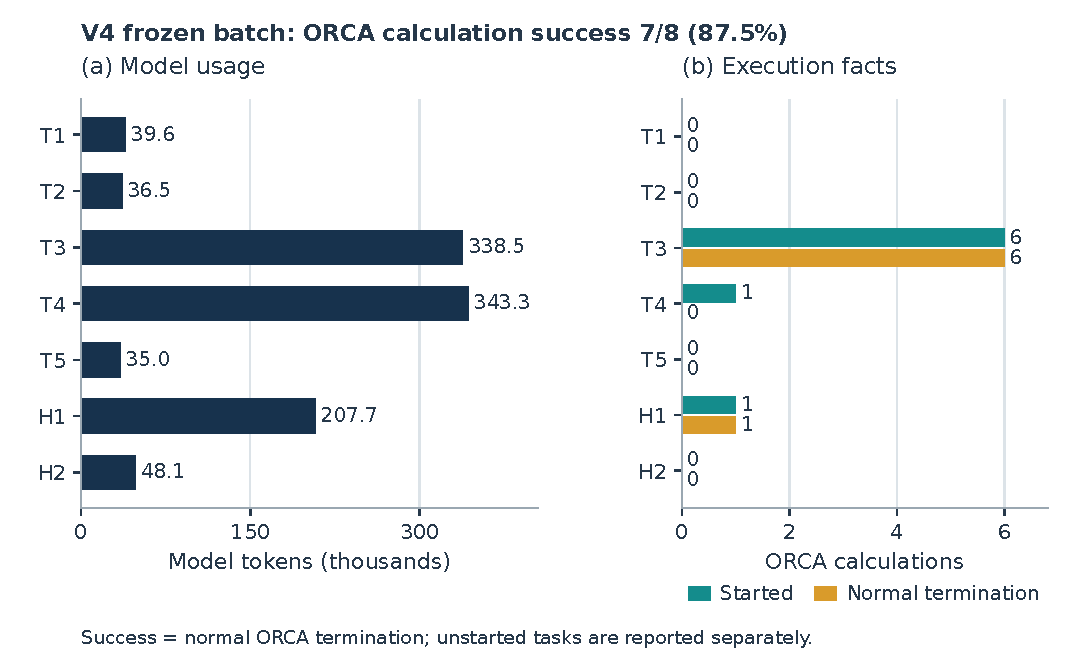
\includegraphics[width=\linewidth]{latest-tasks.pdf}
\caption{V4 七任务评测的模型 token 用量与 ORCA 执行事实。7 次计算成功来自 T3 六次和 H1 一次，另有 1 次 ORCA 输入失败。}
\label{fig:v4-tasks}
\end{figure}

T3 最能说明运行成功与目标完成的分离。模型修复一次 Python 格式化错误后，六次内部 ORCA 计算正常结束并保存产物。然而，程序自设的时间窗口跳过 $+180^\circ$ 端点，曲线与后续采样加密决定没有完成；实际角度与目标角度也未被独立重算。随后反馈上下文超限，且修复步骤未完整继承原目标路线。因此，即使内部计算正常结束，也缺少支持完整扫描结论的证据。

H1 的 NMR 计算产生了 C、N、H 三核总屏蔽张量及各向同性摘要，但结果返回后的上下文构建失败，使后续提取和核对无法完成。T4 则因 ORCA 输入关键词错误停止，外层程序异常掩盖内部错误信息，模型未能及时定位有效修复入口。其中 H1 的 ORCA 计算成功，后续处理失败应单独归因；T4 则属于 ORCA 输入失败。证据发现和结果消费仍是闭环性能的重要组成部分。

\subsection{成本与跨配置观察}
七任务主评测的执行驱动累计经过时间为 2706.749 s，记录的科学计算经过时间和 CPU 时间分别为 1178.063 s 与 3581.138406 s；因采样覆盖有限，后二者作为观测下界。按实验价表计算的模型费用上界为 0.5735982 USD，不代表实际结算账单。模型成本还包含重复读取和反馈组织，不能将 token 用量直接解释为有效科学推理量。

\begin{figure}[htbp]
\centering
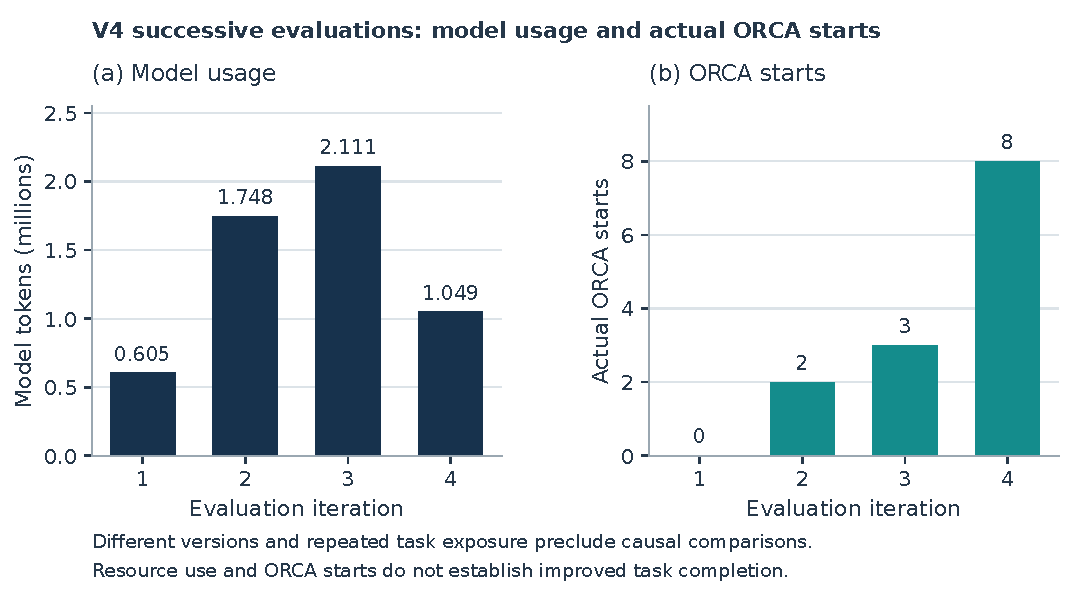
\includegraphics[width=0.96\linewidth]{evaluation-history.pdf}
\caption{V4 四个实验配置的模型 token 用量与 ORCA 启动数。每配置均对相同七题各进行一次评测，配置和任务暴露程度变化，启动次数不直接代表成功次数，故该图仅作描述性统计。}
\label{fig:v4-configurations}
\end{figure}

四个不同配置累计发生 294 次模型调用、5,512,391 tokens 和 13 次 ORCA 启动，完整完成为 0/28 次任务尝试。它们不是同一版本的 28 次独立试验，也不能与 V3 的情境评分合并。历史工作流完成记录作为补充事实保存；本文的计算成果以正常结束调用及其实际数值为依据。后续开发批次已有表 \ref{tab:successful-coverage} 所列六类数值产出，不将其与上述四个冻结配置合并计算成功率。


% !TeX root = ../main.tex
\section{讨论}
\subsection{三种思路的连续性与差异}
V2、V3、V4 分别回答了不同层次的问题。V2 建立实际计算及其证据的可复核性；V3 研究在有限任务范围内，如何将自然语言语义、工具组合和失败修复连接起来；V4 则进一步考察任务算法本身能否由代码生成，并在受控边界内完成开放目标。三者之间存在问题上的递进，但并非在共同任务和相同条件下进行的性能迭代。

V3 的 18/18 包含固定任务、脚本化对话、自动确认与拒绝情境；V4 的计算成功指标针对实际 ORCA 调用，冻结批次为 7/8，后续案例还覆盖更多任务类型。两类分母不同，不能直接解释为性能下降或提升。若要比较版本收益，需要相同原始目标、输入、最低证据、模型与资源，并分别测量完整完成、数值误差和成本。

\subsection{V4 的主要瓶颈是证据链的一致性}
V4 已通过生成程序获得优化结构、振动频率、有限构象单点能量、激发能及核磁屏蔽等真实结果，证明该路线可以支持多种计算任务。当前困难主要出现在从成功计算到后续行动的连接处。失败可归纳为四类：语义与结构化表示不一致、目标条件在层间传递不完整、修复后目标与产物关联丢失，以及反馈上下文和错误发现不足。它们不属于传统 SCF 收敛问题，却可以决定整个科学任务是否完成。

这一结果将约束机制本身纳入研究对象。约束过弱可能使错误目标获得形式通过，过度重复或互不一致的约束又会阻断合法任务。有效改进应在保留科学要求、原始目标与资源边界的同时，减少同一事实的重复表示，并为当前失败提供直接可查询的证据。相关机制的修改需要新的冻结评测；本文新增的计算成功标记仅明确原始 ORCA 执行事实，不改写历史工作流状态。

\subsection{闭环性与科学可靠性}
AutoDFT 为成功与失败均进入后续规划提供了方法参照，多参考自主计算研究则强调电子态身份和覆盖率的重要性。V4 将这些问题组织在单一决策循环中，以统一工具边界约束实际操作。这是架构选择，本文没有单决策者与多角色系统的受控比较，不能据此宣称性能优势。

闭环性也不能仅由存在反馈接口推断。真正有效的反馈应改变后续行动，并持续缩小原始目标的证据缺口。T3 和 H1 均已成功执行 ORCA，同时表明后续反馈组织仍有完善空间。未来评价应考察结果是否被正确消费、必要操作是否实际执行，以及停止时的部分结论是否与已有证据一致。

\subsection{有效性威胁与进一步验证}
实验规模和异质性限制了统计推断。V2 为人工批准的选定成功链，V3 的任务与对话高度限定，V4 主评测每题仅一次；跨版本和跨配置数据不能组成统一成功概率。早期 V3 实验未保存完整执行源码快照，限制严格复现；部分 V4 案例具有人工协助，应与自主评测区分。

科学有效性同样具有范围限制。局部频率检查不证明全局构象最优，候选子集能量排名不证明自由能排序，原始张量存在也不证明目标已完成。固定设置下的数值重复性支持可重复计算，不替代独立高精度或实验参照。本文未验证 V4 的多参考求解能力，也未将指定隔离配置的测试扩展为普遍安全保证。

进一步研究应首先建立同配置的重复试验和未暴露任务集，再对科学输出引入独立参考或确定性复核。针对 V4，可分别检验目标条件统一、修复关联保持和反馈压缩的贡献；扫描任务需要检查端点与实际几何，跨环境比较需要检查条件和共同几何，张量任务需要检查单位及坐标变换。由此将“可以生成程序”的证据推进为“可以稳定完成科学目标”的证据。


% !TeX root = ../main.tex
\section{结论}
本文按 V2、V3、V4 的顺序研究 BG6022 在自主量子化学计算中的三种思路。V2 通过受控工作流建立可复核计算链，V3 在有限任务与对话情境中实现语义参与、工具组合和有界修复，V4 将现场生成代码纳入证据约束闭环，使任务表达从预定义工具扩展至程序化算法。

V4 是本研究的重点。单决策循环、目标与计划分离、统一 ORCA 执行以及结果资格分层形成了受控开放任务的方法基础。现有证据在 T1--T5 与 H1 六类任务中保存了成功 ORCA 计算与实际数值，包括乙醇的无虚频优化结构、正己烷有限候选能量、正丁烷六个约束优化点、丙酮五态激发、两种基组下的环境电子能差和 HCN 屏蔽张量。原冻结批次 8 次启动中 7 次计算成功，成功比例为 87.5\%；H2 尚无极化率数值。这些结果支持代码生成路线的跨任务执行能力，后续研究应进一步完善几何核查、结果提取、完整交付与重复试验。

\paragraph{数据与材料可用性}
支撑本文图表的结构化数据、来源校验信息、绘图程序与 LaTeX 源文件作为补充材料提供。本文对既有实验作回顾性分析，本次文档修订未启动新的计算实验，补充数值来自已保存的后续开发批次。部分早期记录的完整执行快照与独立数值参考不可获得，相应限制已在实验评价中说明。架构示意图由 GPT Image 辅助绘制，六幅量化图由记录数据直接计算生成。

\medskip
\renewcommand{\refname}{参考文献}
\begingroup
\footnotesize
\linespread{1.05}\selectfont
\interlinepenalty=10000
% !TeX root = main.tex
% Bibliographic metadata verified on 2026-10-21.
% 31 scholarly references and 1 official documentation reference.
% DOI, arXiv, publisher and official proceedings records are listed in
% sources-bibliography.json. Preprints are explicitly identified.
\begin{thebibliography}{99}
\setlength{\itemsep}{0.25em}

\bibitem{hk}
P. Hohenberg and W. Kohn.
Inhomogeneous Electron Gas.
\emph{Physical Review} \textbf{136}, B864--B871 (1964).
\href{https://doi.org/10.1103/PhysRev.136.B864}{doi:10.1103/PhysRev.136.B864}.

\bibitem{ks}
W. Kohn and L. J. Sham.
Self-Consistent Equations Including Exchange and Correlation Effects.
\emph{Physical Review} \textbf{140}, A1133--A1138 (1965).
\href{https://doi.org/10.1103/PhysRev.140.A1133}{doi:10.1103/PhysRev.140.A1133}.

\bibitem{react}
S. Yao, J. Zhao, D. Yu, et al.
ReAct: Synergizing Reasoning and Acting in Language Models.
\emph{The Eleventh International Conference on Learning Representations (ICLR)} (2023).
\href{https://openreview.net/forum?id=WE_vluYUL-X}{OpenReview: WE\_vluYUL-X};
\href{https://doi.org/10.48550/arXiv.2210.03629}{预印本 doi:10.48550/arXiv.2210.03629}.

\bibitem{toolformer}
T. Schick, J. Dwivedi-Yu, R. Dessì, et al.
Toolformer: Language Models Can Teach Themselves to Use Tools.
\emph{Advances in Neural Information Processing Systems} \textbf{36}, 68539--68551 (2023).
\href{https://doi.org/10.52202/075280-2997}{doi:10.52202/075280-2997}.

\bibitem{reflexion}
N. Shinn, F. Cassano, A. Gopinath, et al.
Reflexion: Language Agents with Verbal Reinforcement Learning.
\emph{Advances in Neural Information Processing Systems} \textbf{36}, 8634--8652 (2023).
\href{https://doi.org/10.52202/075280-0377}{doi:10.52202/075280-0377}.

\bibitem{chemcrow}
A. M. Bran, S. Cox, O. Schilter, et al.
Augmenting large language models with chemistry tools.
\emph{Nature Machine Intelligence} \textbf{6}, 525--535 (2024).
\href{https://doi.org/10.1038/s42256-024-00832-8}{doi:10.1038/s42256-024-00832-8}.

\bibitem{coscientist}
D. A. Boiko, R. MacKnight, B. Kline, et al.
Autonomous chemical research with large language models.
\emph{Nature} \textbf{624}, 570--578 (2023).
\href{https://doi.org/10.1038/s41586-023-06792-0}{doi:10.1038/s41586-023-06792-0}.

\bibitem{orca2020}
F. Neese, F. Wennmohs, U. Becker, et al.
The ORCA quantum chemistry program package.
\emph{The Journal of Chemical Physics} \textbf{152}, 224108 (2020).
\href{https://doi.org/10.1063/5.0004608}{doi:10.1063/5.0004608}.

\bibitem{orca6}
F. Neese.
Software Update: The ORCA Program System---Version 6.0.
\emph{WIREs Computational Molecular Science} \textbf{15}, e70019 (2025).
\href{https://doi.org/10.1002/wcms.70019}{doi:10.1002/wcms.70019}.

\bibitem{opipaper}
T. Tetenberg, H. Neugebauer, C. Plett, et al.
ORCA Meets Python---The ORCA Python Interface OPI.
\emph{Journal of Chemical Theory and Computation} \textbf{22}, 4951--4967 (2026).
\href{https://doi.org/10.1021/acs.jctc.5c02141}{doi:10.1021/acs.jctc.5c02141}.

\bibitem{ase}
A. H. Larsen, J. J. Mortensen, J. Blomqvist, et al.
The atomic simulation environment---a Python library for working with atoms.
\emph{Journal of Physics: Condensed Matter} \textbf{29}, 273002 (2017).
\href{https://doi.org/10.1088/1361-648X/aa680e}{doi:10.1088/1361-648X/aa680e}.

\bibitem{aiida}
G. Pizzi, A. Cepellotti, R. Sabatini, et al.
AiiDA: automated interactive infrastructure and database for computational science.
\emph{Computational Materials Science} \textbf{111}, 218--230 (2016).
\href{https://doi.org/10.1016/j.commatsci.2015.09.013}{doi:10.1016/j.commatsci.2015.09.013}.

\bibitem{atomate2}
A. M. Ganose, H. Sahasrabuddhe, M. Asta, et al.
Atomate2: modular workflows for materials science.
\emph{Digital Discovery} \textbf{4}, 1944--1973 (2025).
\href{https://doi.org/10.1039/D5DD00019J}{doi:10.1039/D5DD00019J}.

\bibitem{cclib}
N. M. O'Boyle, A. L. Tenderholt, and K. M. Langner.
cclib: A library for package-independent computational chemistry algorithms.
\emph{Journal of Computational Chemistry} \textbf{29}, 839--845 (2008).
\href{https://doi.org/10.1002/jcc.20823}{doi:10.1002/jcc.20823}.

\bibitem{autodft}
P. Yang, Z. Zhang, Y. Li, et al.
AutoDFT: A Closed-Loop Multi-Agent Framework for Autonomous DFT Calculations.
\emph{arXiv preprint}, arXiv:2605.26179v2 (2026), 2026年6月4日版本.
\href{https://doi.org/10.48550/arXiv.2605.26179}{doi:10.48550/arXiv.2605.26179}.

\bibitem{multirefagent}
V. C. Lee and J. M. Rondinelli.
Can Autonomous LLM Agents Execute Multireference Quantum Chemistry Calculations?
\emph{arXiv preprint}, arXiv:2609.13357v1 (2026), 2026年9月11日版本.
\href{https://doi.org/10.48550/arXiv.2609.13357}{doi:10.48550/arXiv.2609.13357}.

\bibitem{casscf}
B. O. Roos, P. R. Taylor, and P. E. M. Siegbahn.
A complete active space SCF method (CASSCF) using a density matrix formulated super-CI approach.
\emph{Chemical Physics} \textbf{48}, 157--173 (1980).
\href{https://doi.org/10.1016/0301-0104(80)80045-0}{doi:10.1016/0301-0104(80)80045-0}.

\bibitem{nevpt2}
C. Angeli, R. Cimiraglia, S. Evangelisti, et al.
Introduction of \emph{n}-electron valence states for multireference perturbation theory.
\emph{The Journal of Chemical Physics} \textbf{114}, 10252--10264 (2001).
\href{https://doi.org/10.1063/1.1361246}{doi:10.1063/1.1361246}.

\bibitem{avas}
E. R. Sayfutyarova, Q. Sun, G. K.-L. Chan, et al.
Automated Construction of Molecular Active Spaces from Atomic Valence Orbitals.
\emph{Journal of Chemical Theory and Computation} \textbf{13}, 4063--4078 (2017).
\href{https://doi.org/10.1021/acs.jctc.7b00128}{doi:10.1021/acs.jctc.7b00128}.

\bibitem{questdb}
P.-F. Loos, M. Boggio-Pasqua, A. Blondel, et al.
QUEST Database of Highly-Accurate Excitation Energies.
\emph{Journal of Chemical Theory and Computation} \textbf{21}, 8010--8033 (2025).
\href{https://doi.org/10.1021/acs.jctc.5c00975}{doi:10.1021/acs.jctc.5c00975}.

\bibitem{pbe}
J. P. Perdew, K. Burke, and M. Ernzerhof.
Generalized Gradient Approximation Made Simple.
\emph{Physical Review Letters} \textbf{77}, 3865--3868 (1996).
\href{https://doi.org/10.1103/PhysRevLett.77.3865}{doi:10.1103/PhysRevLett.77.3865}.

\bibitem{becke}
A. D. Becke.
Density-functional thermochemistry. III. The role of exact exchange.
\emph{The Journal of Chemical Physics} \textbf{98}, 5648--5652 (1993).
\href{https://doi.org/10.1063/1.464913}{doi:10.1063/1.464913}.

\bibitem{lyp}
C. Lee, W. Yang, and R. G. Parr.
Development of the Colle--Salvetti correlation-energy formula into a functional of the electron density.
\emph{Physical Review B} \textbf{37}, 785--789 (1988).
\href{https://doi.org/10.1103/PhysRevB.37.785}{doi:10.1103/PhysRevB.37.785}.

\bibitem{def2}
F. Weigend and R. Ahlrichs.
Balanced basis sets of split valence, triple zeta valence and quadruple zeta valence quality for H to Rn: Design and assessment of accuracy.
\emph{Physical Chemistry Chemical Physics} \textbf{7}, 3297--3305 (2005).
\href{https://doi.org/10.1039/B508541A}{doi:10.1039/B508541A}.

\bibitem{d3}
S. Grimme, J. Antony, S. Ehrlich, et al.
A consistent and accurate \emph{ab initio} parametrization of density functional dispersion correction (DFT-D) for the 94 elements H--Pu.
\emph{The Journal of Chemical Physics} \textbf{132}, 154104 (2010).
\href{https://doi.org/10.1063/1.3382344}{doi:10.1063/1.3382344}.

\bibitem{tddft}
E. Runge and E. K. U. Gross.
Density-Functional Theory for Time-Dependent Systems.
\emph{Physical Review Letters} \textbf{52}, 997--1000 (1984).
\href{https://doi.org/10.1103/PhysRevLett.52.997}{doi:10.1103/PhysRevLett.52.997}.

\bibitem{cpcm}
M. Cossi, N. Rega, G. Scalmani, et al.
Energies, structures, and electronic properties of molecules in solution with the C-PCM solvation model.
\emph{Journal of Computational Chemistry} \textbf{24}, 669--681 (2003).
\href{https://doi.org/10.1002/jcc.10189}{doi:10.1002/jcc.10189}.

\bibitem{gfn2}
C. Bannwarth, S. Ehlert, and S. Grimme.
GFN2-xTB---An Accurate and Broadly Parametrized Self-Consistent Tight-Binding Quantum Chemical Method with Multipole Electrostatics and Density-Dependent Dispersion Contributions.
\emph{Journal of Chemical Theory and Computation} \textbf{15}, 1652--1671 (2019).
\href{https://doi.org/10.1021/acs.jctc.8b01176}{doi:10.1021/acs.jctc.8b01176}.

\bibitem{crest}
P. Pracht, F. Bohle, and S. Grimme.
Automated exploration of the low-energy chemical space with fast quantum chemical methods.
\emph{Physical Chemistry Chemical Physics} \textbf{22}, 7169--7192 (2020).
\href{https://doi.org/10.1039/C9CP06869D}{doi:10.1039/C9CP06869D}.

\bibitem{fair}
M. D. Wilkinson, M. Dumontier, I. J. Aalbersberg, et al.
The FAIR Guiding Principles for scientific data management and stewardship.
\emph{Scientific Data} \textbf{3}, 160018 (2016).
\href{https://doi.org/10.1038/sdata.2016.18}{doi:10.1038/sdata.2016.18}.

\bibitem{r2scan3c}
S. Grimme, A. Hansen, S. Ehlert, and J.-M. Mewes.
r$^{2}$SCAN-3c: A "Swiss army knife" composite electronic-structure method.
\emph{The Journal of Chemical Physics} \textbf{154}, 064103 (2021).
\href{https://doi.org/10.1063/5.0040021}{doi:10.1063/5.0040021}.

\bibitem{opi}
FACCTs.
\emph{ORCA Python Interface (OPI) 2.0 Documentation}.
官方技术文档，访问日期：2026年10月21日.
\url{https://www.faccts.de/docs/opi/2.0/docs/}.

\end{thebibliography}

\endgroup
\end{document}
